%%%%%%%%%%%%%%%%%%%MAIN_OPTIONS%%%%%%%%%%%%%%%%%%%
\documentclass[a4paper, 14pt]{article}

%% Работа с русским языком
\usepackage{cmap}					% поиск в PDF
\usepackage{hyperref}				% гиперссылки
\usepackage[warn]{mathtext} 		% русские буквы в формулах
\usepackage[T2A]{fontenc}			% кодировка
\usepackage[utf8]{inputenc}			% кодировка исходного текста
\usepackage[english,russian]{babel}	% локализация и переносы

%% Дополнительная работа с математикой
\usepackage{amsfonts,amssymb,amsthm,mathtools} % AMS
\usepackage{amsmath}
\usepackage{icomma} % "Умная" запятая: $0,2$ --- число, $0, 2$ --- перечисление

%% Номера формул
%\mathtoolsset{showonlyrefs=true} % Показывать номера только у тех формул, на которые есть \eqref{} в тексте.

%%FONTS_Packadges
\usepackage{euscript} % Шрифт Евклид
\usepackage{mathrsfs} % Красивый матшрифт

%% Свои команды
\DeclareMathOperator{\sgn}{\mathop{sgn}}

%% Перенос знаков в формулах (по Львовскому)
\newcommand*{\hm}[1]{#1\nobreak\discretionary{}
	{\hbox{$\mathsurround=0pt #1$}}{}}

%%% Работа с картинками
\usepackage{graphicx}  % Для вставки рисунков
\graphicspath{{pictures/}{images2/}}  % папки с картинками
\setlength\fboxsep{3pt} % Отступ рамки \fbox{} от рисунка
\setlength\fboxrule{1pt} % Толщина линий рамки \fbox{}
\usepackage{wrapfig} % Обтекание рисунков и таблиц текстом
\usepackage[section]{placeins}
\usepackage{subcaption}

%% Работа с таблицами
\usepackage{array,tabularx,tabulary,booktabs} % Дополнительная работа с таблицами
\usepackage{longtable}  % Длинные таблицы
\usepackage{multirow} % Слияние строк в таблице

%%Links
\hypersetup{
	colorlinks=true,
	linkcolor=black,
	filecolor=magenta,      
	urlcolor=blue,
}

%%% Программирование
\usepackage{etoolbox} % логические операторы

%%% Страница
\usepackage{extsizes} % Возможность сделать 14-й шрифт
\usepackage{geometry} % Простой способ задавать поля
\geometry{top=25mm}
\geometry{bottom=35mm}
\geometry{left=20mm}
\geometry{right=20mm}
\usepackage{indentfirst}
%
\usepackage{fancyhdr} % Колонтитулы
\pagestyle{fancy}
\renewcommand{\headrulewidth}{0mm}  % Толщина линейки, отчеркивающей верхний колонтитул
%\lfoot{Нижний левый}
%\rfoot{Нижний правый}
%\rhead{Верхний правый}
%\chead{Верхний в центре}
%\lhead{Верхний левый}
% \cfoot{Нижний в центре} % По умолчанию здесь номер страницы

\usepackage{setspace} % Интерлиньяж
%\onehalfspacing % Интерлиньяж 1.5
%\doublespacing % Интерлиньяж 2
%\singlespacing % Интерлиньяж 1

\usepackage{multicol,caption}

\newenvironment{Figure}
{\par\medskip\noindent\minipage{\linewidth}}
{\endminipage\par\medskip}

\usepackage{enumitem}
\usepackage{amssymb}
\usepackage{xcolor}
%%% Зачеркнутый текст
\usepackage[normalem]{ulem}



\begin{document}

	\title{		\textbf{\textit{Победит \#398}} 
		
		Сегментация зерен сплава WC-Co готовыми инструментами}

	\author{$ Д.Г. Каграманян^1, Д.Ю. Камалова^2, Б.Б. Страумал^3, Л.Н. Щур^4$}
	\date{\today}
	\maketitle
	
	\hfill
	\begin{minipage}{1\textwidth}
		\flushleft
		$^1$исследователь,dgkagramanyan@edu.hse.ru\\
		$^2$исследователь,dyukamalova@edu.hse.ru \\
		$^3$соруководитель,straumal@issp.ac.ru\\
		$^4$руководитель,levshchur@gmail.com\\
		
		
		
	\end{minipage}%




	
	\section{Аннотация}

	Мы работаем с фотографиями микростуктурам (рис. \ref{fig:original}) WC-Co с различным процентным соотношением вольфрама, углерода и кобальта. 
	Каждая вариация сплава отличается своими характеристиками: твердостью, пластичностью, 
	хрупкостью, средним размером зерен, количеством пустот и тд.

	Исходное изображение состоит из двух частей. Первая половина микроструктуры получена на основе отраженных электронов, а другая - на основе поглощенных. Каждая из них отражает особенности микроструктуры по-своему. 

	\begin{figure}[h]
		\center{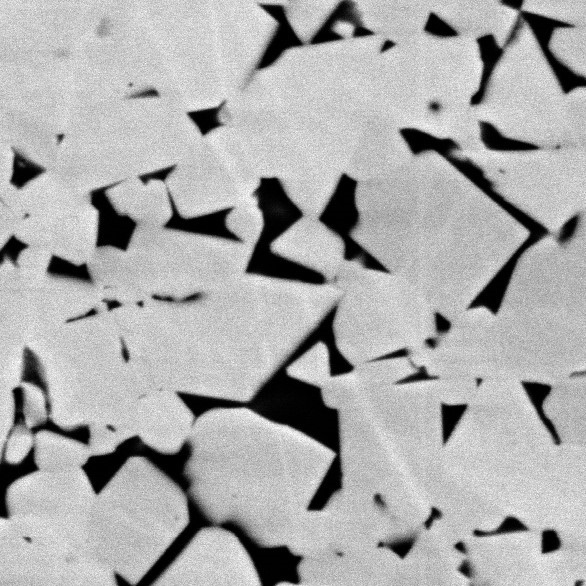
\includegraphics[scale=0.2]{segment_images/original}}
		\caption{Фотография микроструктуры Ultra-Co11-2}
		\label{fig:original}
	\end{figure}


	\section{Задача}
	
	Для исследования сплава требуется качественно выделить все характеристики и особенности 
	кристаллической решетки по фотографиям микрострктур. 
	
	Для этого нужно сегментировать каждое зерно карбида вольфрама и каждую пустоту, состоящую из кобальта, чтобы в дальнейшем определить площадь зерен, периметр, углы и тд. 
	

	\section{Предобработка изображений}
	
	Фотографии микростоструктур связки WC-Co имеют видимый уровннь шума. Особенно сильно 
	это видно при оптическом увеличении зерен. Зашумленность выражается в виде 
	множества неупорядоченных белых и серых пикселей на поверхности зерна (рис. \ref{ris:noise}). 
	

	Чтобы снизить уровень шума воспользуемся медианным фильтром. Его особенность в том, что он хорошо справляется со своей задачей и при этом не делает границы объектов менее четкими. 
	
	Также наложим левую и правую части фотографии, чтобы увеличить контрасность признаков (рис. \ref{fig:combine2} ).
	

	\begin{figure}[h]
	\begin{center}
		\begin{minipage}[h]{0.4\linewidth}
			\center{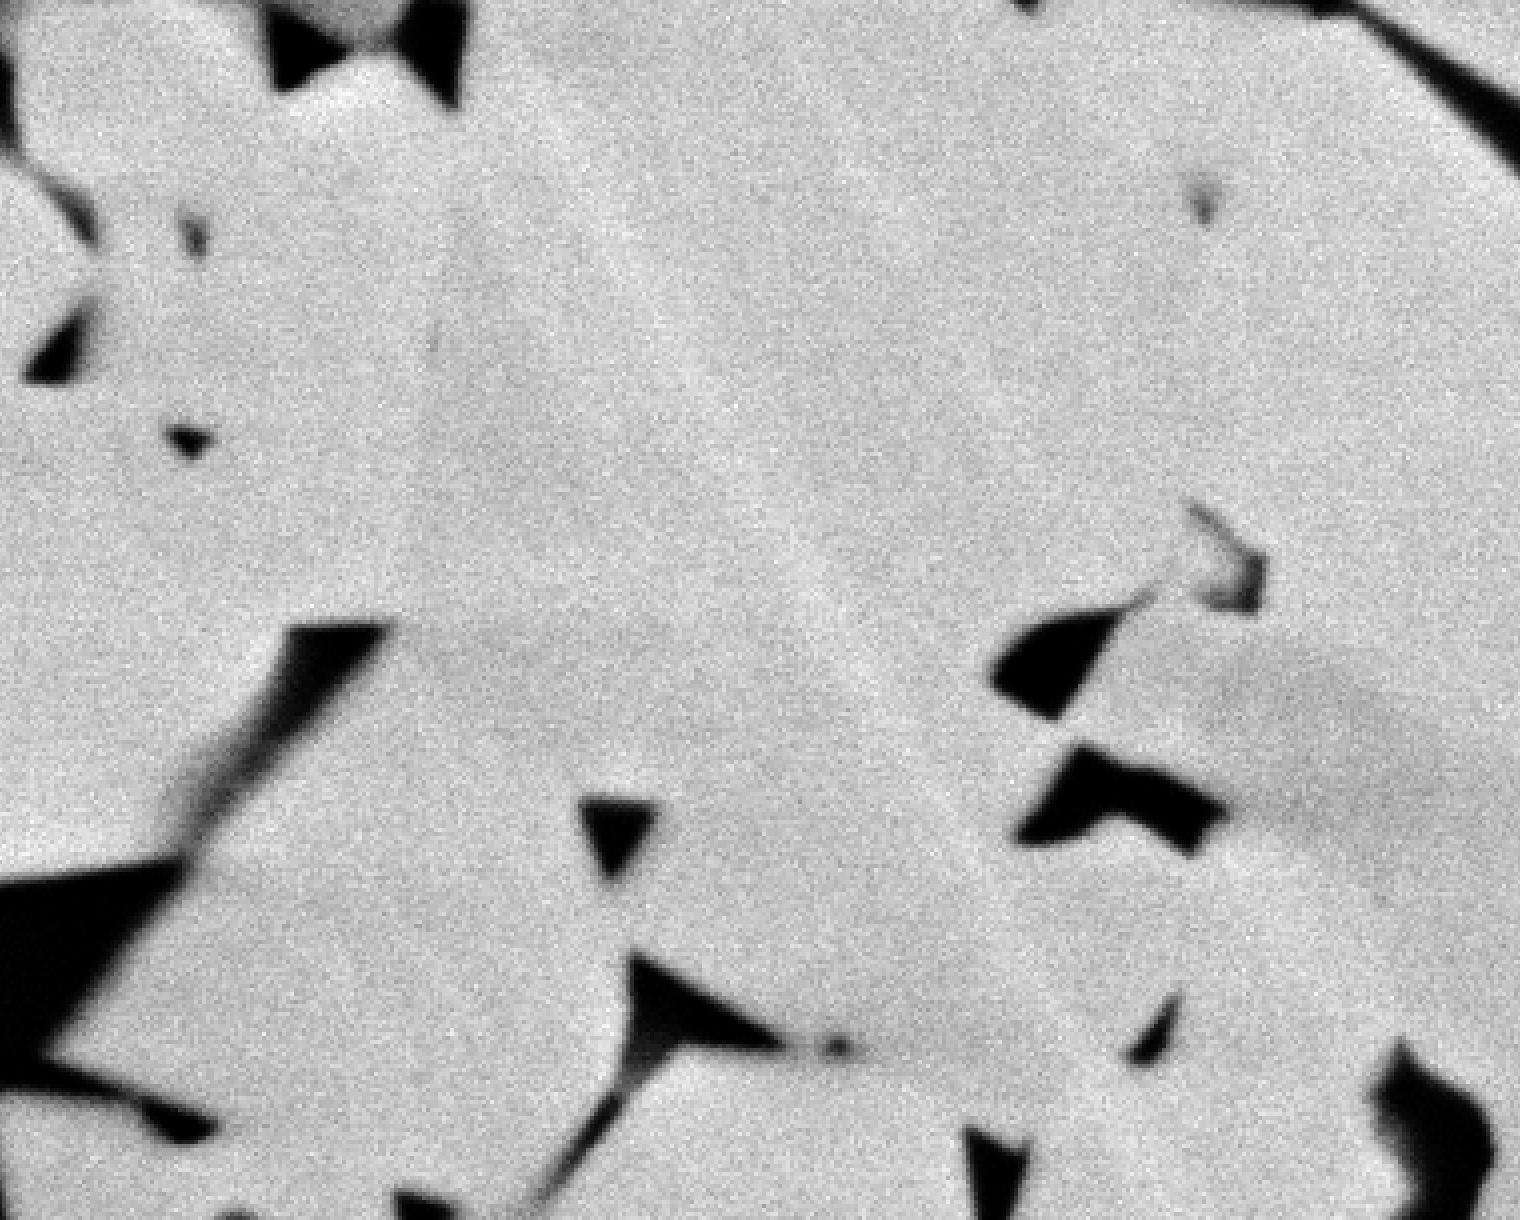
\includegraphics[scale=0.2]{segment_images/grain_zoom}}
		\caption{Зашумленные зерна карбида вольфрама}
		\label{ris:noise}
		\end{minipage}
		\hfill
		\begin{minipage}[h]{0.4\linewidth}
		\center{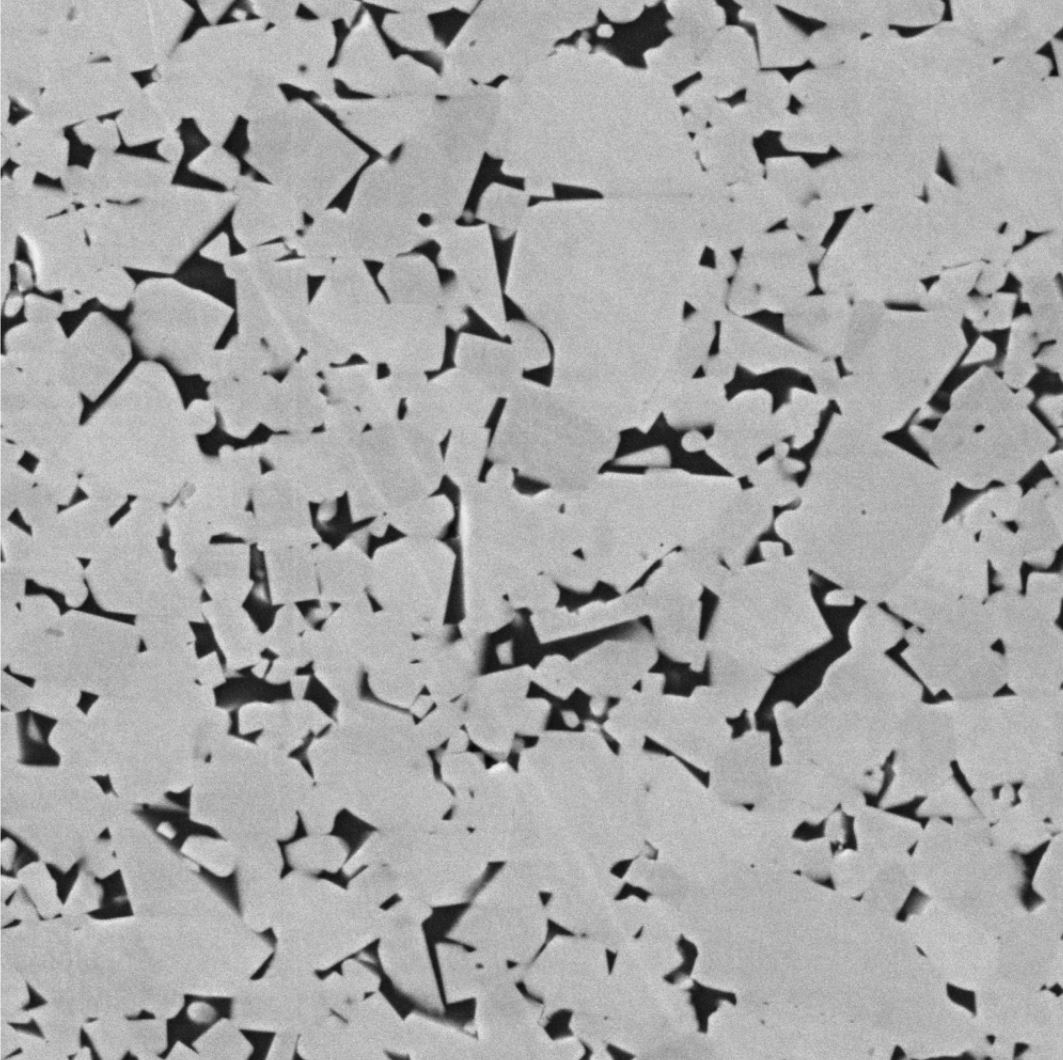
\includegraphics[scale=0.25]{segment_images/combine2}}
\caption{Совмещенное изображения в поглощенных и отраженных электронах}
\label{fig:combine2}
		\end{minipage}
	\end{center}
\end{figure}

	
	\section{Применение сегментации}
	Существует множество готовых алгортимов для сегментации объектов на изображении. 
	Рассмотрим самые популярные:
	
		\begin{itemize}
		
		\item  watershed - изображение рассматривается 
		как поверхность \cite{habr_watershed}. Начиная от глобального минимума, изображение будет "заполняться"  водой. 
		По мере поднятия уровня "воды" выделяются локальные минимумы .
		
		Существует также улучшенная версия алгоритма.
		Можно заранее задать прмерные районы минимумов, или иными словами маркеры. 
		Их можно задать вручную, картой расстояний пикселей , 
		картой градиентов  и тд;
		
		\item k-means -  разделение множества входных векторов на группы (кластеры)
		 по степени «схожести» друг на друга \cite{habr_k-means}. Алгоритм стремится минимизировать суммарное квадратичное отклонение точек кластеров от центров этих кластеров ; 
		
		\item floodfill -  выделение однородных по цвету регионов при помощи заливки \cite{habr_watershed}. Алгоритм будет объединять пиксели в один сегмент (заливая их одним цветом), если они попадают в указанный диапазон;
		
		\item felzenswalb -  кластеризация минимально охватывающего дерева \cite{felz_link}. 
		Алгоритм не сообщает нам точное количество кластеров, на которые будет разделено изображение. Он будет генерировать столько кластеров, сколько он считает нужным для этого. 
		Применим после метод k-means , это может улучшить качество работы сегментации;
		
		\item DBSCAN - алгоритм группирует вместе точки, которые тесно расположены , помечая как выбросы точки, которые находятся одиноко в областях с малой плотностью \cite{dbscan}.
		

		
	\end{itemize}

	\section{Результаты}
	
		Почти все алгоритмы дали похожую картину
	
	\begin{itemize}
		
		\item простой watershed - нет результата (рис. \ref {fig:watershed}) ;
		
		\item watershed с маркерами edt - хорошее виделение структур на карте расстояний,
		но итогового результата нет (рис. \ref {fig:watershed_edt});
		
		\item k-means -  нет результата (рис. \ref {fig:k-means});
		
		\item floodfill - нет результата;
		
		\item felzenswalb - нет результата, алгоритм сегментирует не объекты, а шумы (рис. \ref {fig:felz});  
		
		\item felzenswalb и k-means - нет результата,
		алгоритм сегментирует не объекты, а шумы  (рис. \ref{fig:felz_k-means});  
		
		\item watershed с градиентыми маркерами - отличное выделение границ пустот, 
		результат - довольно точная сегментация пространства между зернами (рис. \ref {fig:watershed_grad});
		
		\item DBSCAN - нет результата.
		
		
		
		
	\end{itemize}
	
	\begin{figure}[h]
		\begin{center}
			\begin{minipage}[h]{0.4\linewidth}
					\center{
\includegraphics[scale=0.65]{segment_images/watershed}}
				\caption{Watershed}
				\label{fig:watershed}
			\end{minipage}
			\hfill
			\begin{minipage}[h]{0.4\linewidth}
					\center{
\includegraphics[scale=0.5]{segment_images/k-means}}
			\caption{K-means}
			\label{fig:k-means}
			\end{minipage}
		\end{center}
	\end{figure}
	
	


	\begin{figure}[h]
		\center{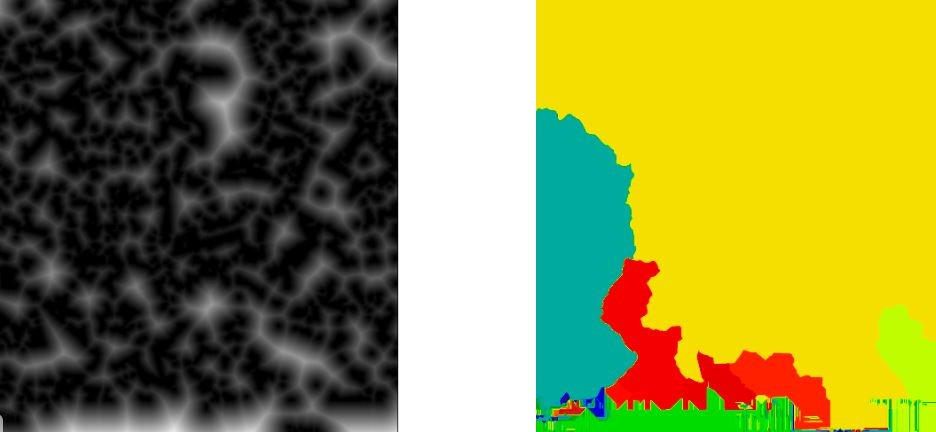
\includegraphics[scale=0.57]{segment_images/watershed_edt}}
		\caption{Watershed с маркерами edt (Euclidean distance transform)}
		\label{fig:watershed_edt}
	\end{figure}

		\begin{figure}[h]
		\begin{center}
			\begin{minipage}[h]{0.4\linewidth}
				\center{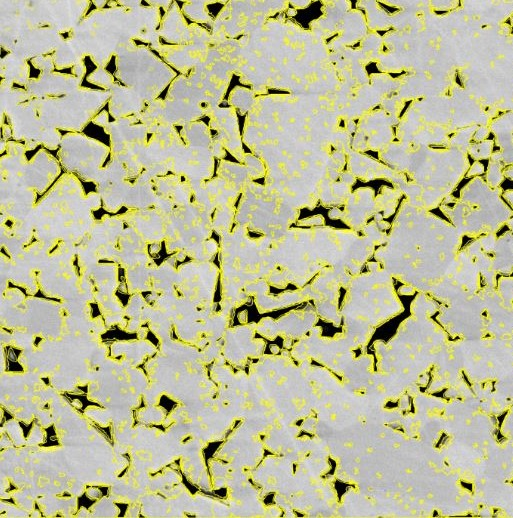
\includegraphics[scale=0.4]{segment_images/felz}}
			\caption{Felzenszwalb}
			\label{fig:felz}
			\end{minipage}
			\hfill
			\begin{minipage}[h]{0.4\linewidth}
					\center{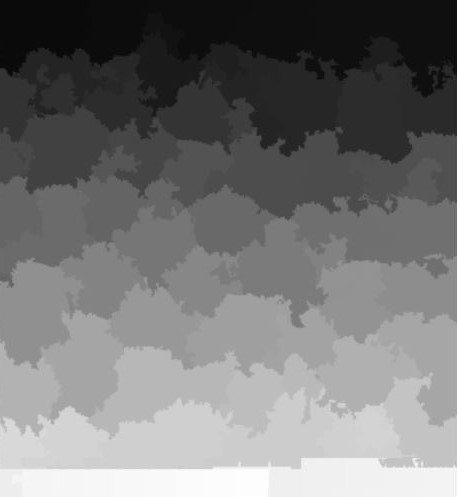
\includegraphics[scale=0.4]{segment_images/felz+k-means}}
				\caption{Felzenszwalb+k-means}
				\label{fig:felz_k-means}
			\end{minipage}
		\end{center}
	\end{figure}

	
	\begin{figure}[h]
		\center{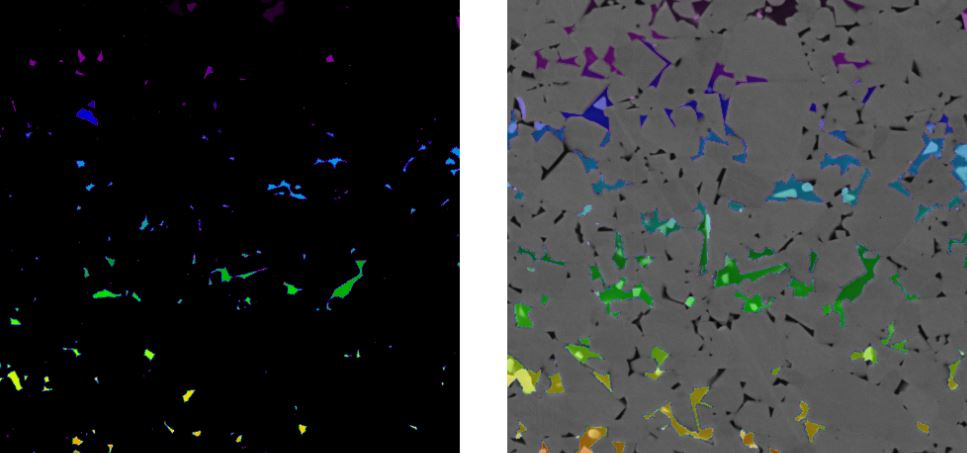
\includegraphics[scale=0.6]{segment_images/watershed_grad}}
		\caption{Watershed с градиентными маркерами}
		\label{fig:watershed_grad}
	\end{figure}

	
	 
	\section{Трудности}

	\begin{figure}[h]
	\center{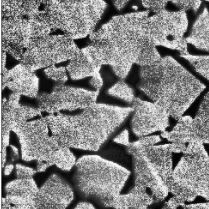
\includegraphics[scale=1]{segment_images/noised}}
	\caption{Микроструктура с увеличенной контрастностью}
	\label{fig:noised}
\end{figure}



	
	
 
 		Смежные границы зерен неразличимы. При детальном осмотре выявлено, что значения пикселей границы 
	 ниже или равны уровню шума на изображении.
	 
	 Увеличение контрасности изображения не делает границы зерен более видимыми, а наоборот, значительно 
	 повышает уровень шума (рис. \ref{fig:noised}).
	 		


	\section{Новый метод сегментации}


	Так как методы сегментации на основе обнаружения граний объектов результата не дали, 
	то попробуем применить другой метод, основанный пустотах между зернами.
	
	Для сегментации зерен построим граф G=(V,E), где вершины V - углы пустот, а E - ребра, соединяющие вершины. 
	
	Изначально все вершины графа G изолированы. Итеративно пройдемся по всем вершинам, соединяя их друг с другом по специальному правилу
	
	\begin{itemize}
		\item количество ребер у вершины меньше или равно 4;
		
		\item ребро не может проходить через пустоту. Разрешается только по ее границе;
		

		\item ребро не может проходить сквозь другую вершину.
		
	\end{itemize}
	
	\textbf{Первый проход.}
	Сначала все углы пустот маркируются вершинами. Соединяются ребрами те вершины, 
	которых связывает одна пустота. Соединение происходит только с теми вершинами,
	 которые находятся на одной стороне границы. 
	
	\textbf{Второй проход.}  
	Пройдемся по вершинам, у котороых уже есть 2 ребра. Для создания 3-го ребра пустим луч  противоположно углу 
	2-х ребер, по направлению биссектрисы. Исключаются вершины с углами 90 градусов. Третьим ребром вершины становится другая вершина, максимально \textbf{близкая} к лучу. Длина луча не может быть \textbf{больше}, чем сумма 2х ребер с учетом их угла (тупой угол
	- больше длина луча, острый угол - меньше длина).
	
	Если такой вершны нет, то от каждой из 2-х ребер строятся нормали, по которым пускаеются лучи до
	обнаружения новой вершины в определенном \textbf{раудиусе}.
	
	
	\textbf {Третий проход.} В случае с прямыми углами из вершины по направлению прямого угла пускается луч. Если он пересекает зерно и затем проходит 
	рядом с реброом, паралелльным ему, то искомая вершина соединяется с ближайшей вершиной найденного паралелльного ребра.
	
	Цель алгоритма - пройтись по всем вершинам, у которых есть 2 ребра. 
	
	
	\begin{figure}[h]
		\center{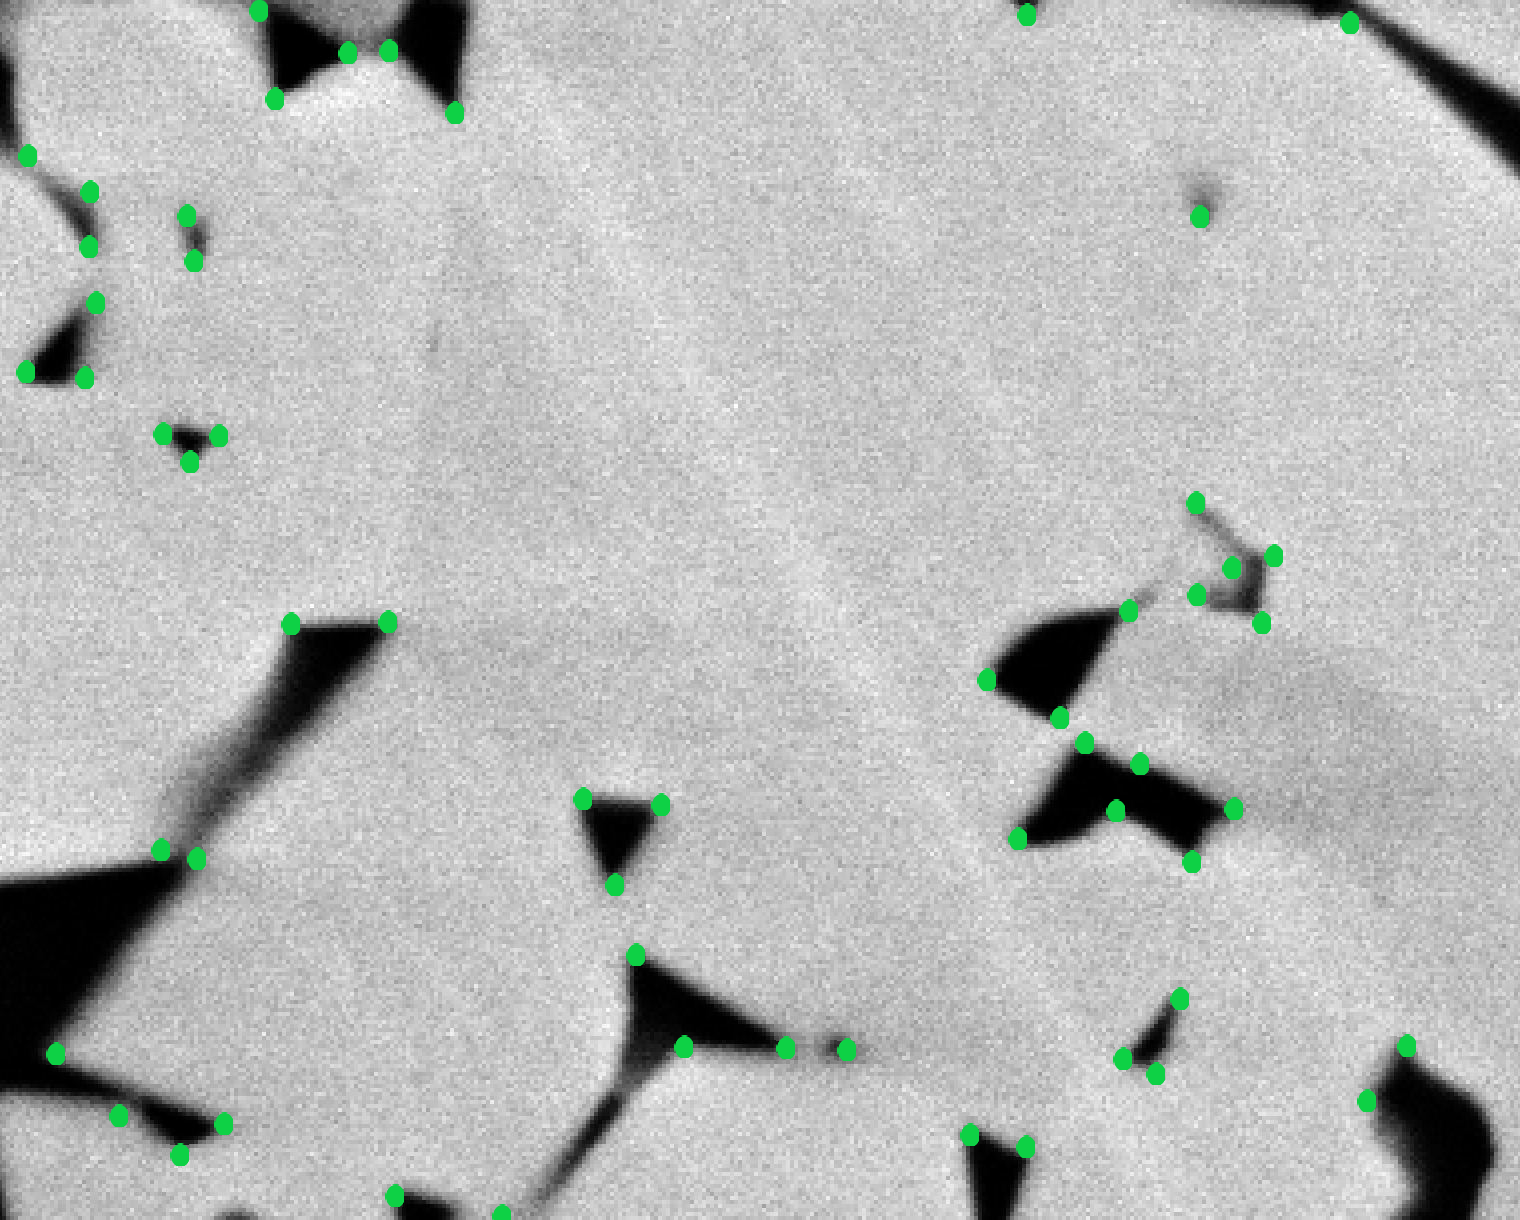
\includegraphics[scale=0.2]{segment_images/zoom_dots}}
		\caption{Этап 1.1, разметка вершин (зеленые точки) пустот }
		\label{ris:image}
	\end{figure}

	\begin{figure}[h]
	\center{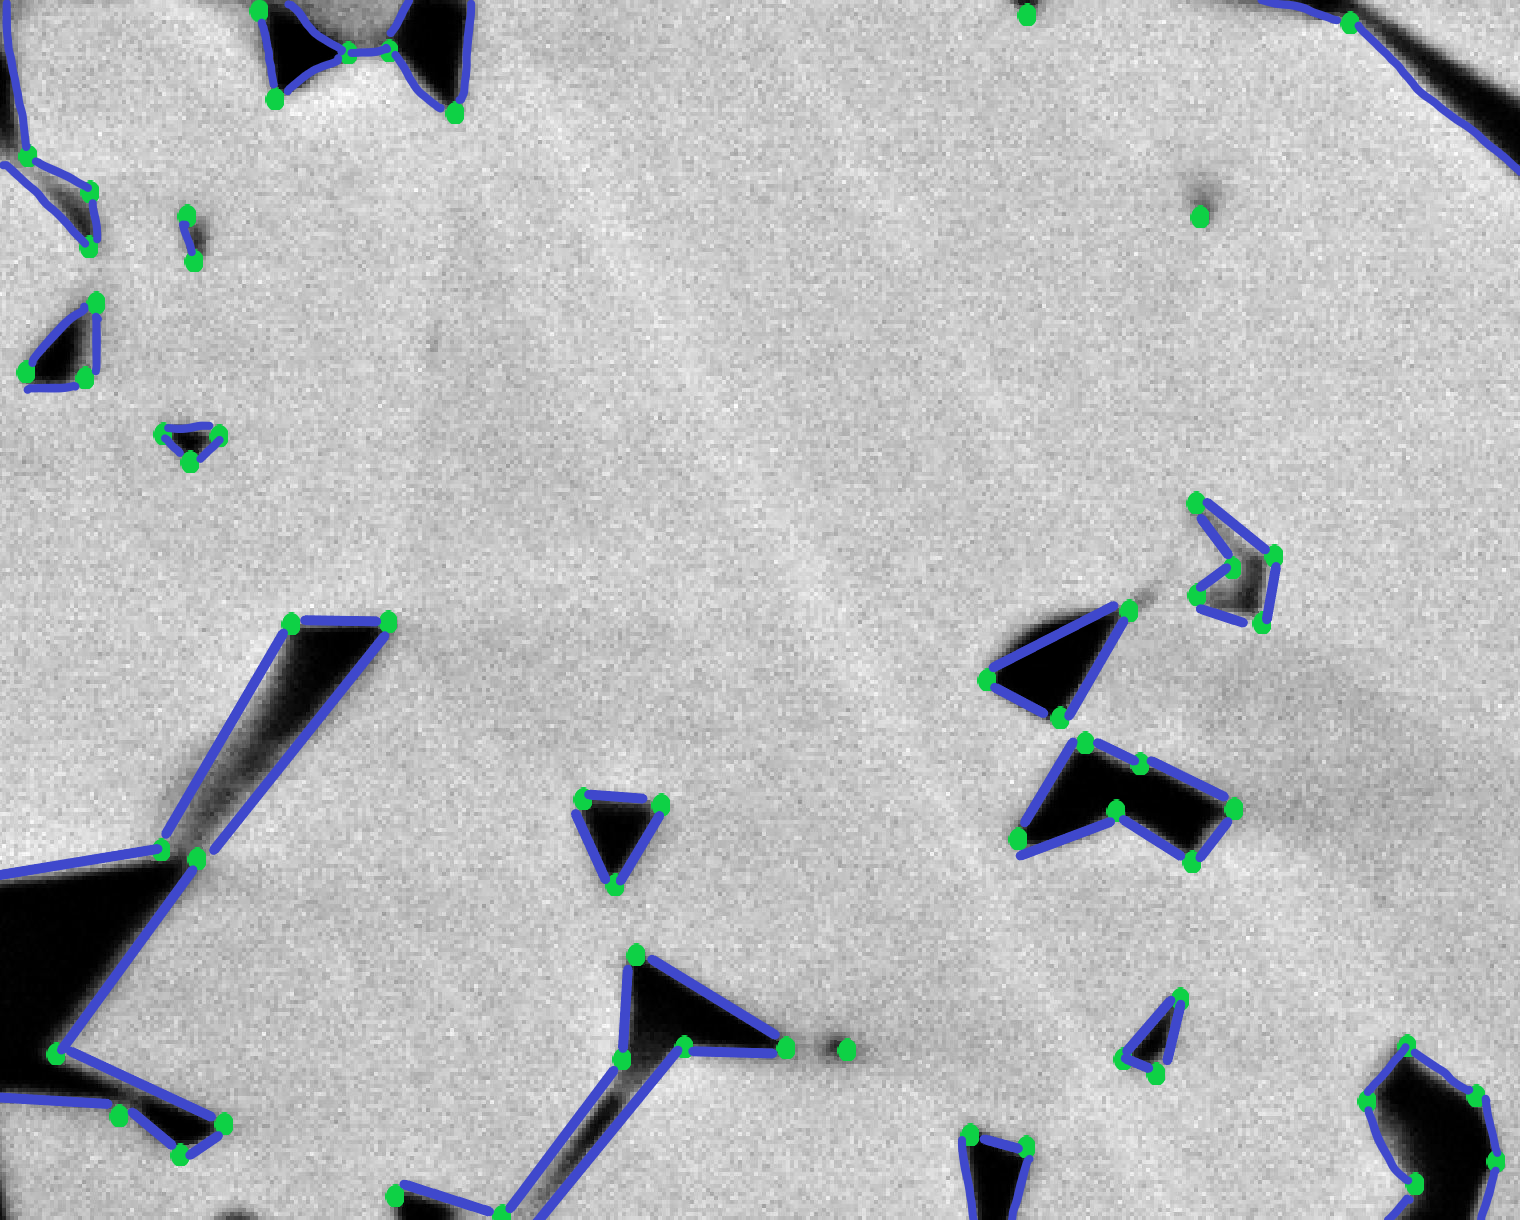
\includegraphics[scale=0.2]{segment_images/zoom_lines_1}}
	\caption{Этап 1.2, Построение подграфов пустот (ребра синие) }
	\label{ris:image}
	\end{figure}

	\begin{figure}[h]
		\center{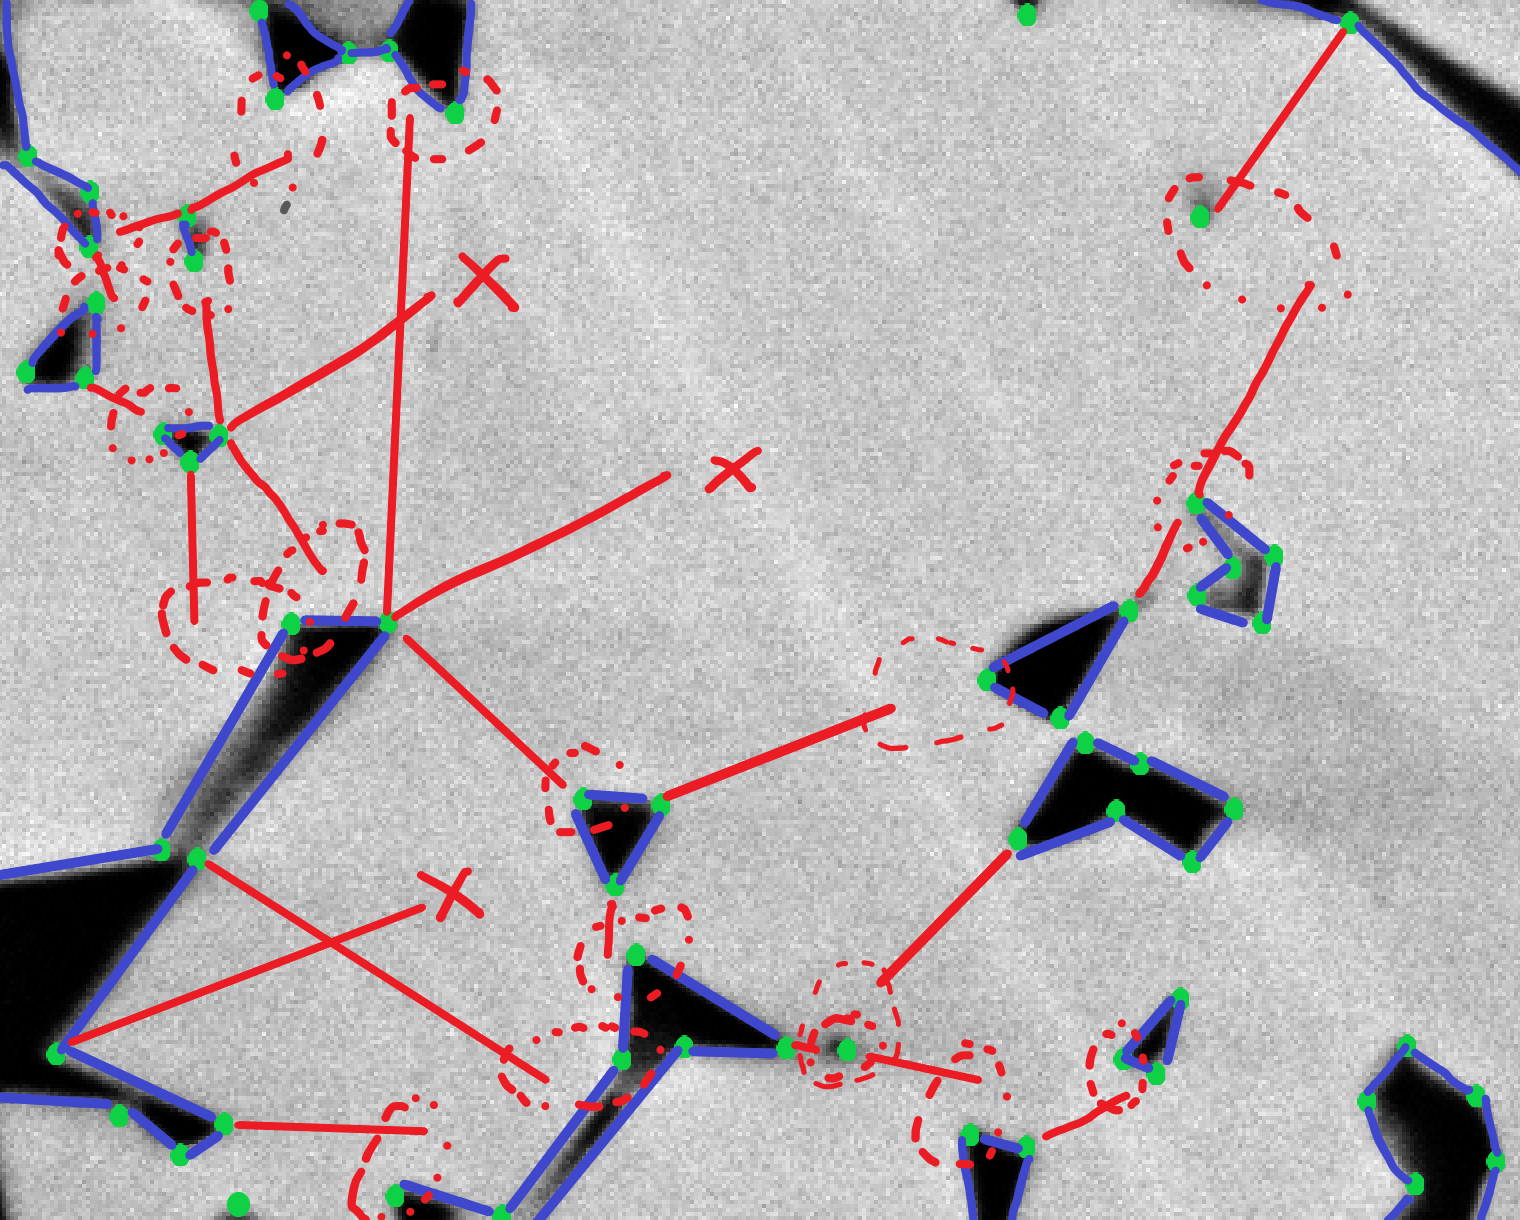
\includegraphics[scale=0.2]{segment_images/zoom_lines_2}}
		\caption{Этап 2 и 3, обход всех вершин и построение дополнительных ребер }
		\label{ris:image}
	\end{figure}
	
	\begin{figure}[h]
		\center{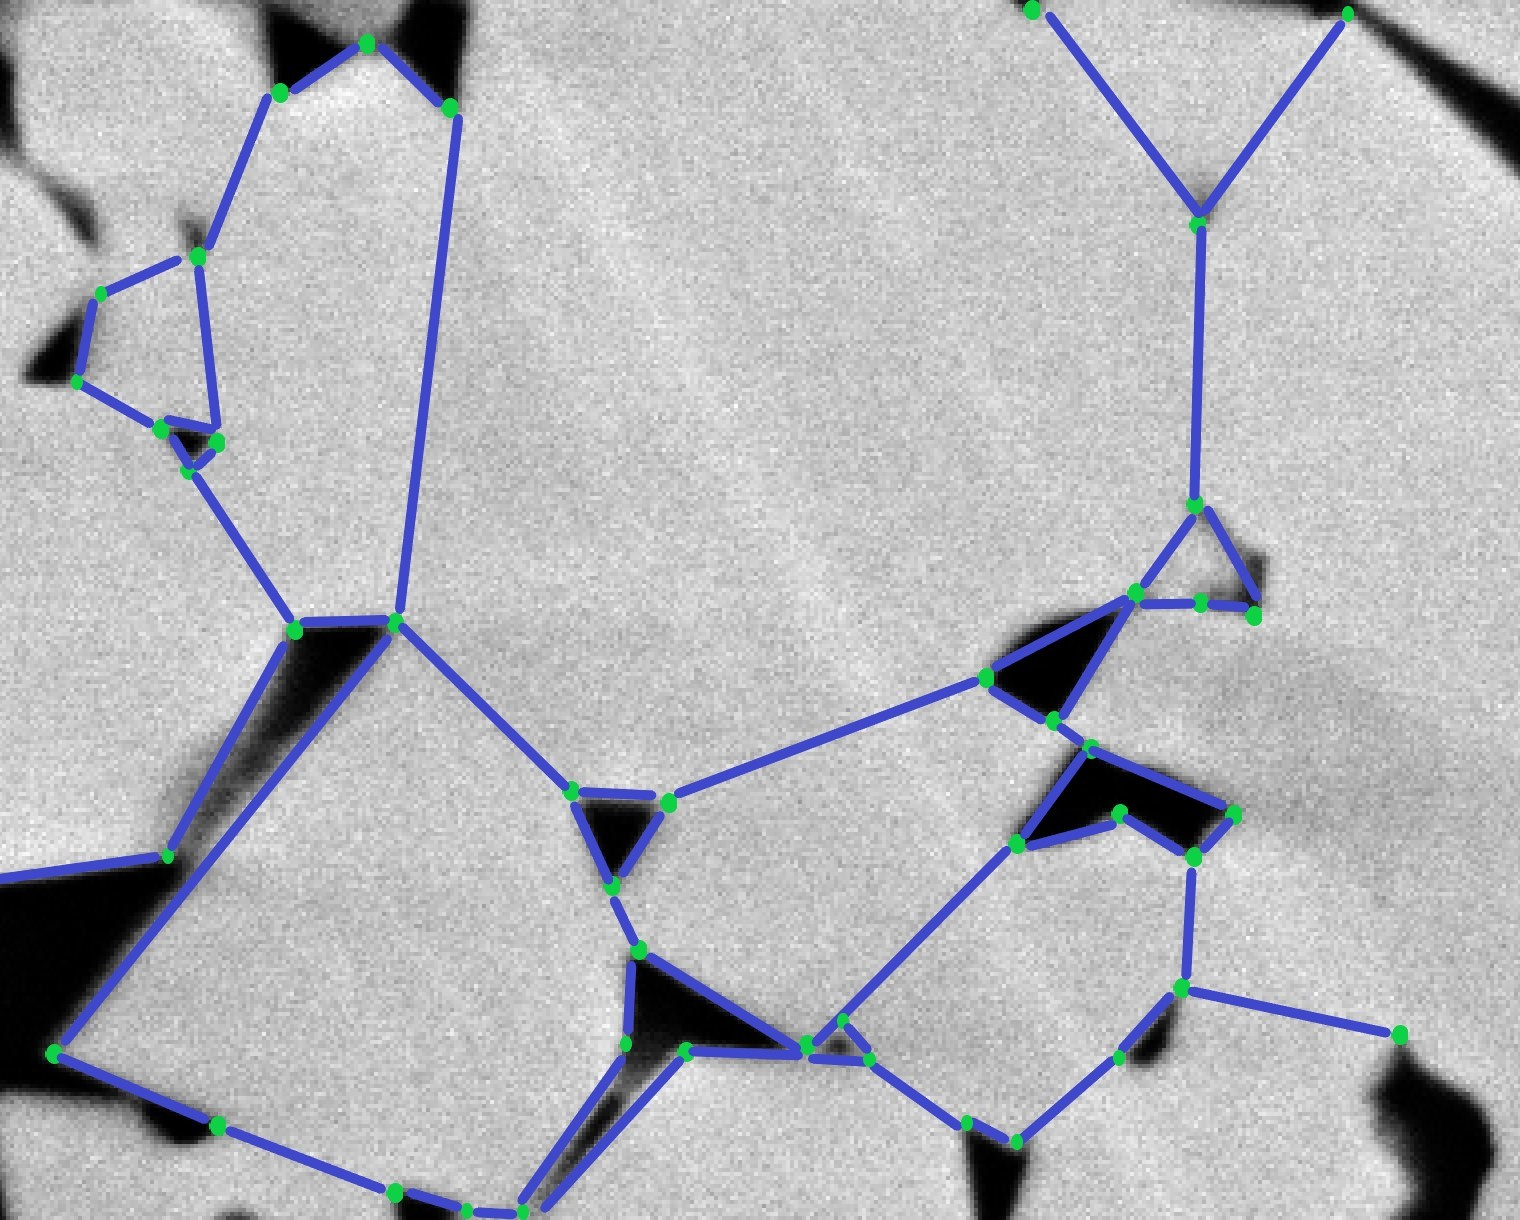
\includegraphics[scale=0.2]{segment_images/grain_zoom_marked_linear}}
		\caption{Получившийся граф G, вершины V - зеленые, ребра E - синие }
		\label{ris:image}
	\end{figure}
	
	\section{Выводы}
	Наложение фотографий на основе 
	поглощенных и отраженных электронов не повышает контрасность изображения. Единственное отличие - 
	на отраженных электронах лучше отображены артефакты (рытвины, ямы).
	
	Готовые алгоритмы сегментации не справляются с сегментацией зерен. Их основные принципы работы - 
	разбиение объектов на классы на основе границ, либо на основе схожести пикселей. У зерен 
	карбида вольфрама смежные границы не различимы, а структура кристиллов однородная, то есть все зерна 
	визуально схожи по цветовой гамме. 
	
	Ручная разметка дает хорошее пнимание структуры связки WC-Co. При внимательном зрительном анализе сладывается впечатление, что выделение зерна происходит на основе едва видимых смежных 
	границ. В действительности человеческий мозг "сам" достраивает необходимые линии на основе пустот между зернами. 
	
	Это хорошо видно на рисунке \ref{fig:grain_red}. Выделенными красным цветом это области, где с большой 
	вероятностью проходит граница зерна. В большинстве таких областей нет даже едва видимой границы, однако 
	соседние пустоты подсказывают о ее наличии. 
	
	Приведенный в \ref{solve} главе способ сегментации на основе построения графа может решить поставленную задачу. 
	
	\begin{figure}[h]
		\center{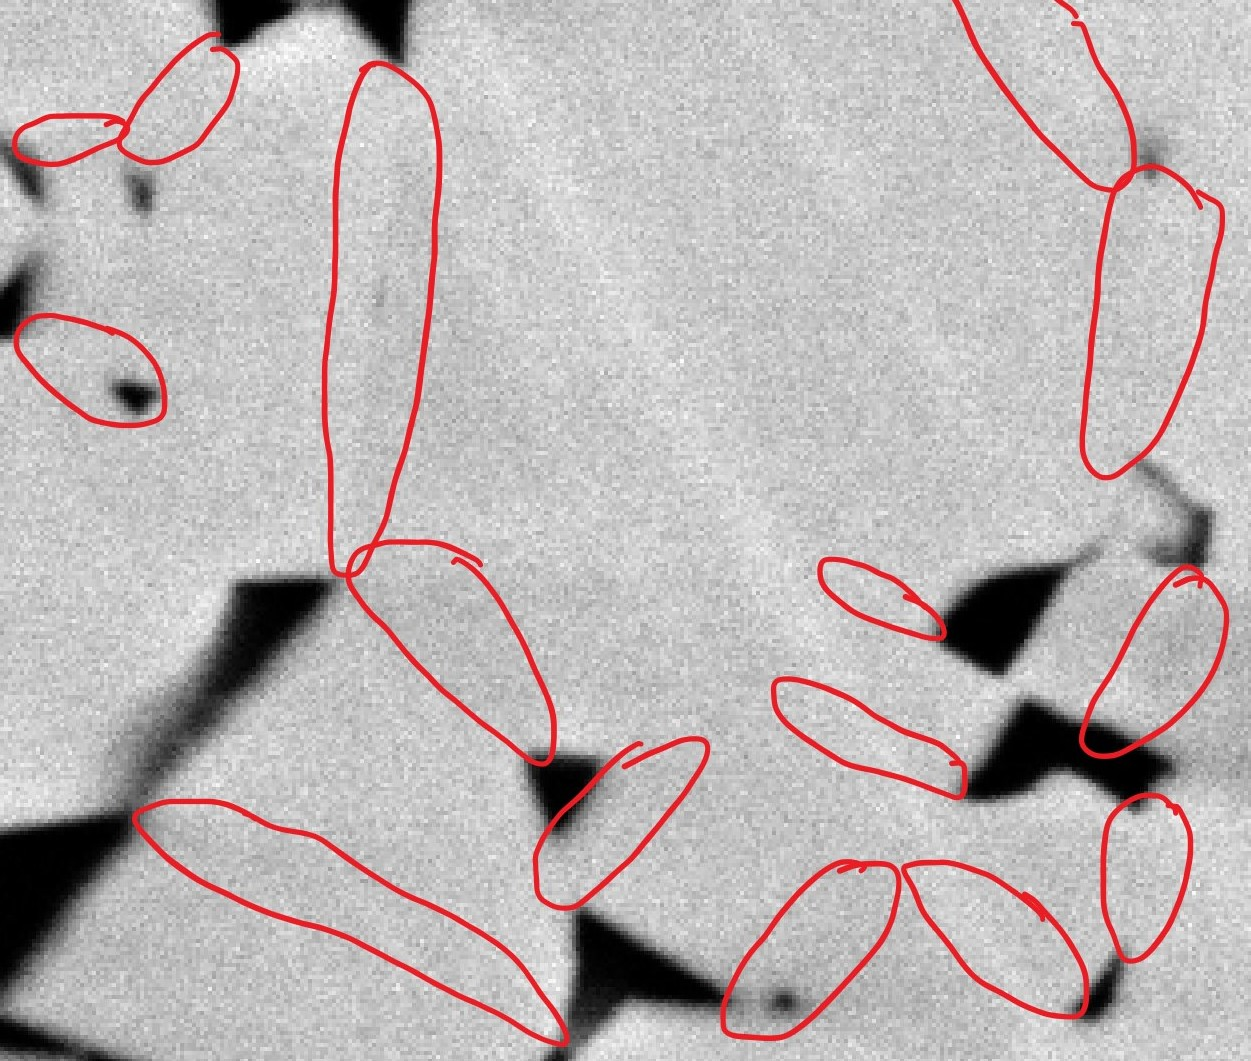
\includegraphics[scale=0.23]{segment_images/grain_zoom_marked}}
		\caption{Микроструктура с выделенными границами}
		\label{fig:grain_red}
	\end{figure}
	
%далее сам список используевой литературы
\begin{thebibliography}{}
	\bibitem{habr_watershed}  NastyaL  -  \href{https://habr.com/ru/company/intel/blog/266347/}{Обзор алгоритмов сегментации}
	\bibitem{habr_k-means} sashaeve - 
	 \href{https://habr.com/ru/post/67078/}{Кластеризация: алгоритмы k-means и c-means}
	\bibitem{felz_link}  Pedro F. Felzenszwalb, Daniel P. Huttenlocher  -  
	\href{https://people.cs.uchicago.edu/~pff/papers/seg-ijcv.pdf}{Efficient Graph-Based Image Segmentation}
	\bibitem{dbscan} Siarshai
	 - \href{https://habr.com/ru/post/322034/}{Интересные алгоритмы кластеризации, часть вторая: DBSCAN}
\end{thebibliography}
	



	
\end{document}